\documentclass[12pt]{article}
\usepackage[utf8]{inputenc}
\usepackage[spanish,activeacute]{babel}
\usepackage{amsmath}
\usepackage{geometry}
\usepackage{fancyhdr}
\usepackage{graphicx}
\usepackage{hyperref}
\hypersetup{
    colorlinks=true,
    linkcolor=blue,
    urlcolor=blue
}
\usepackage{xcolor}
\usepackage{enumitem}
\usepackage{framed}
\usepackage{tcolorbox}
\usepackage{draftwatermark} % Paquete para la marca de agua

% Configuración de la marca de agua
\SetWatermarkText{Ingeniería Social} % Texto de la marca de agua
\SetWatermarkScale{3} % Tamaño de la marca de agua
\SetWatermarkColor[gray]{0.9} % Color y transparencia de la marca de agua

% Configuración de márgenes
\geometry{left=2cm, right=2cm, top=2.5cm, bottom=2.5cm}

% Configuración del encabezado y pie de página
\pagestyle{fancy}
\fancyhf{}
\fancyhead[L]{
\includegraphics[width=2.5cm]{logo2.jpeg}}
\fancyhead[C]{\textbf{\sffamily Capstone Project: Analitiks Spa}}
\fancyfoot[C]{\thepage}

% Colores personalizados
\definecolor{primary}{RGB}{34, 85, 136}
\definecolor{secondary}{RGB}{0, 128, 128}
\definecolor{questionbg}{RGB}{240, 240, 240}

\begin{document}

% Título principal
\begin{center}
    \vspace*{8cm}
    {\Huge \textbf{\sffamily Informe de avance}}\\[0.5em]
\end{center}

\begin{center}
    
\includegraphics[width=8cm]{ANALITIKS.png}
\end{center}

\begin{center}
    \vspace{9cm}
    \textcolor{secondary}{\textbf{Santiago de Chile}}\\
    \textit{Viernes, 30 de septiembre de 2022}
    \vspace{1cm}
\end{center}


\newpage



% Índice
\tableofcontents
\newpage

% Resumen Ejecutivo
\section{Ingeniería Social}

\subsection{¿Qué es la Ingeniería Social?}
\noindent
La ingeniería social es una técnica de manipulación psicológica que se utiliza para engañar a las personas y obtener información confidencial. Es una de las herramientas más utilizadas en el mundo de la ciberseguridad, ya que no se necesita ser un experto en tecnología para entender cómo funciona. Imaginate que alguien te llama por teléfono haciéndose pasar por un representante de tu banco. Te hablan de un problema con tu cuenta y, con tono amigable, te piden que confirmes tus datos personales o inclusive tu contraseña. Aunque parezca totalmente creible, pueden ganarse tu confianza con palabras, manipulando tus emociones con el fin de obtener información personal y confidencial.\\
De eso se trata la ingeniería social, el arte de manipular a las personas para que entreguen información privada sin darse cuenta. El entender la ingeniería social no solo nos ayuda a protegernos de estos engaños, sino también a reconocer cómo los ciberdelincuentes aprovechan nuestra psicología para violar nuestra seguridad.\\
\begin{center}
    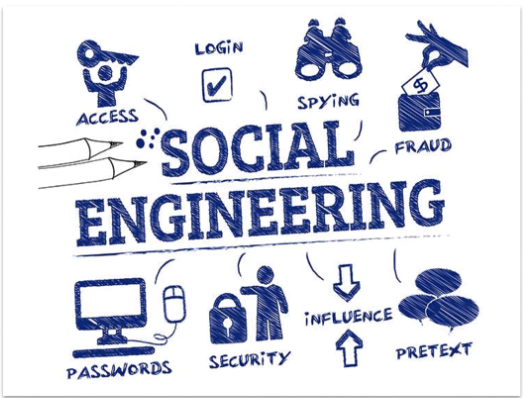
\includegraphics[width=15cm]{ingsocial.png}
\end{center}

\newpage

\section{Tipos de Ingeniería Social}

\subsection{Social Engineer Toolkit (SET)}
\noindent
El Social Engineer Toolkit (SET) es un conjunto útil de herramientas que, además de ser de código abierto, es una de las más populares en el mundo de la ciberseguridad. Es ampliamente utilizado por testers de penetración y equipos de seguridad (los famosos Red Teams) para evaluar la seguridad de una organización imitando ataques de ingeniería social dirigiros al personal.\\
SET ofrece una amplia gama de métodos para realizar ataques, como puede ser la clonación de sitios web, cargas maliciosas, spear phishing o la creación de medios infectados. Lo anteriormente mencionado son ataques dificiles de defender, ya que se aprovechan de las debilidades humanas ya que son inevitables dentro de una organización.
\subsubsection{Instalación de SET}
\noindent
Para instalar SET, primero debemos clonar el repositorio de GitHub. Para ello, abrimos una terminal y ejecutamos el siguiente comando:
\begin{framed}
\begin{verbatim}
git clone https://github.com/trustedsec/social-engineer-toolkit
\end{verbatim}
\end{framed}
\begin{center}
    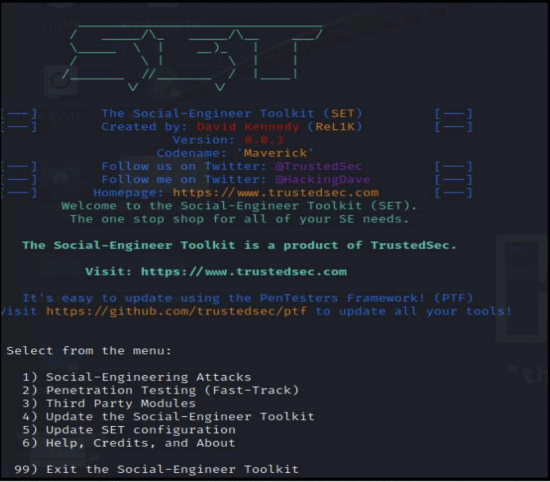
\includegraphics[width=12cm]{set.png}
\end{center}

\newpage
\noindent
Cuando ya estemos dentro del SET, encontraremos diferentes opciones en el menu.

\subsection{Social-Engineer Attacks}
\begin{center}
    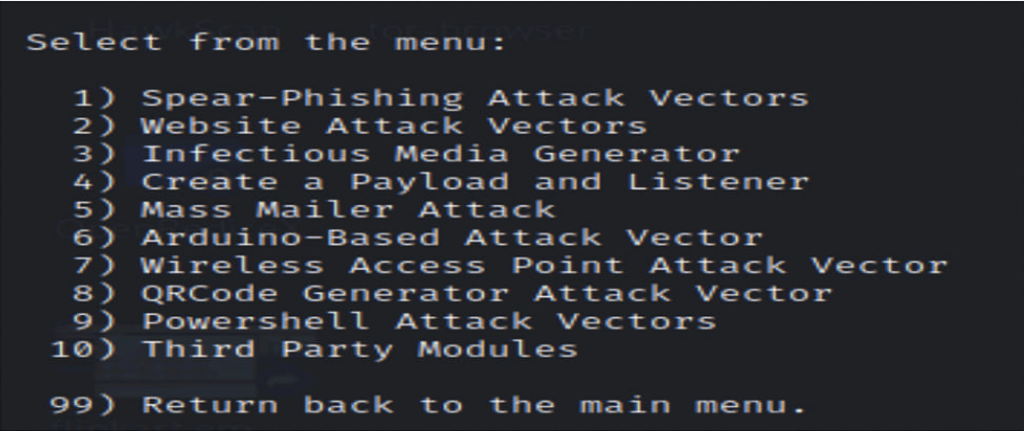
\includegraphics[width=12cm]{sav.png}
\end{center}

\noindent
La primera opción que encontramos en el SET se centra en diferentes vectores de ataque utilizados en la ingeniería social, como puede ser el phishing, la clonación de sitios web, entre otros. Los usuarios pueden usarla para probar y simular varios escenarios de ataque basados en el comportamiento humano.

\subsection{Penetration Testing (Fast-Track)}

\begin{center}
    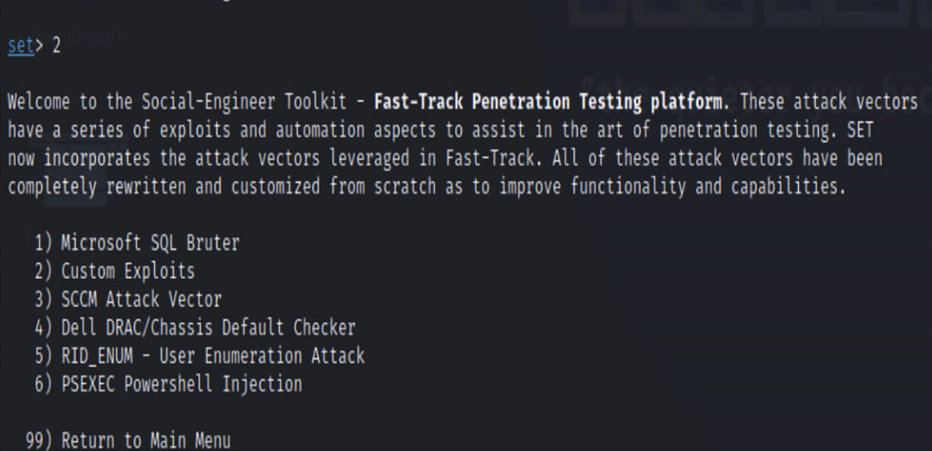
\includegraphics[width=12cm]{pt.png}
\end{center}

\noindent
La segunda opción que encontramos en el SET es el Fast-Track, que es una herramienta que automatiza el proceso de pruebas de penetración, permitiendo identificar rápidamente las vulnerabilidades y aprovechar fallos de seguridad. Es una herramienta muy útil para los equipos de seguridad que buscan identificar y corregir vulnerabilidades en sus sistemas.

\newpage

\subsection{Third Party Modules}

\begin{center}
    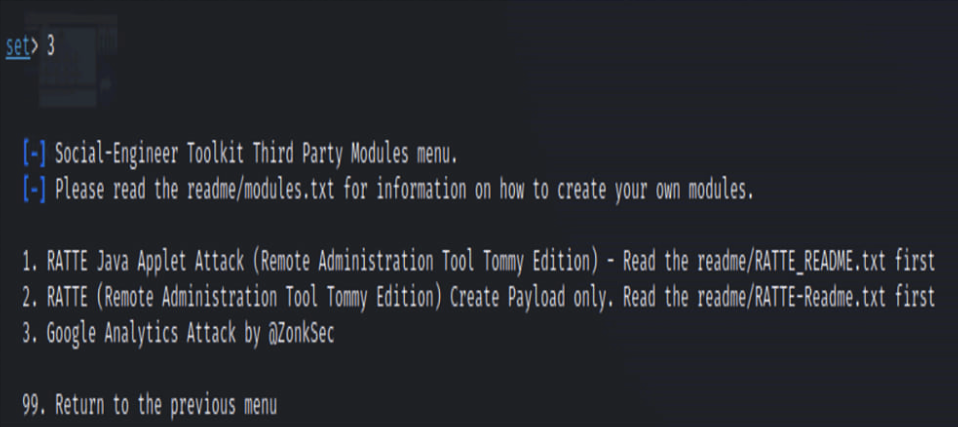
\includegraphics[width=12cm]{tpm.png}
\end{center}

\noindent
La tercera opción que encontramos en el SET es la de los módulos de terceros, que son herramientas adicionales que se pueden instalar para ampliar las capacidades del SET. Estos módulos ofrecen cargas utiles adicionales, exploits y rutas de ataque para el toolkit.

\subsection{Update the Social-Engineer Toolkit}

\noindent
La cuarta opción que encontramos en el SET es la de actualizar el toolkit. Es importante mantener el SET actualizado para asegurarse de que se tengan las últimas actualizaciones y parches de seguridad para garantizar su funcionalidad y confiabilidad.

\subsection{Update SET configuration}

\noindent
Con esta opción puedes editar el archivo de configuración de SET para personalizar la configuración del toolkit y adaptarla a tus necesidades y preferencias.

\subsection{Help, Credits, and About}

\noindent
La última opción que encontramos en el SET es la de ayuda, créditos y acerca de. Esta opción proporciona información sobre cómo utilizar el toolkit, los créditos de los desarrolladores y una descripción general del toolkit.

\newpage

\section{Conclusión}

\noindent
Existen muchas más opciones disponibles además de las mencionadas. Podemos utilizar las herramientas diversas y potentes del invaluable Social Engineer Toolkit (SET) para realizar phishing, recolectar credenciales, clonar sitios web, entre otros.\\
Es siempre importante usar estas herramientas de manera consciente y solo con fines de investigación en seguridad y aprendizaje.

\section{Referencias}


\end{document}
